\documentclass[tikz,border=12pt]{standalone}
\usepackage[T1]{fontenc}
\usepackage{lmodern}
\usetikzlibrary{positioning,arrows.meta,automata}
\definecolor{navy}{HTML}{09234F}\definecolor{blue}{HTML}{384CE3}\definecolor{paid}{HTML}{1F8A63}
\definecolor{held}{HTML}{C27A12}\definecolor{bad}{HTML}{C03A2B}\definecolor{ink}{HTML}{0B0F17}
\tikzset{
  s/.style={draw=navy,line width=.6pt,rounded corners=3pt,fill=white,font=\sffamily\small,minimum width=30mm,minimum height=10mm,align=center},
  ok/.style={s,draw=paid,fill=paid!8},hold/.style={s,draw=held,fill=held!8},no/.style={s,draw=bad,fill=bad!8},wait/.style={s,draw=blue,fill=blue!8},
  arr/.style={-{Stealth[length=2.2mm]},draw=navy,line width=.55pt},
  e/.style={font=\sffamily\scriptsize,fill=white,inner sep=1.5pt,align=center}
}
\begin{document}
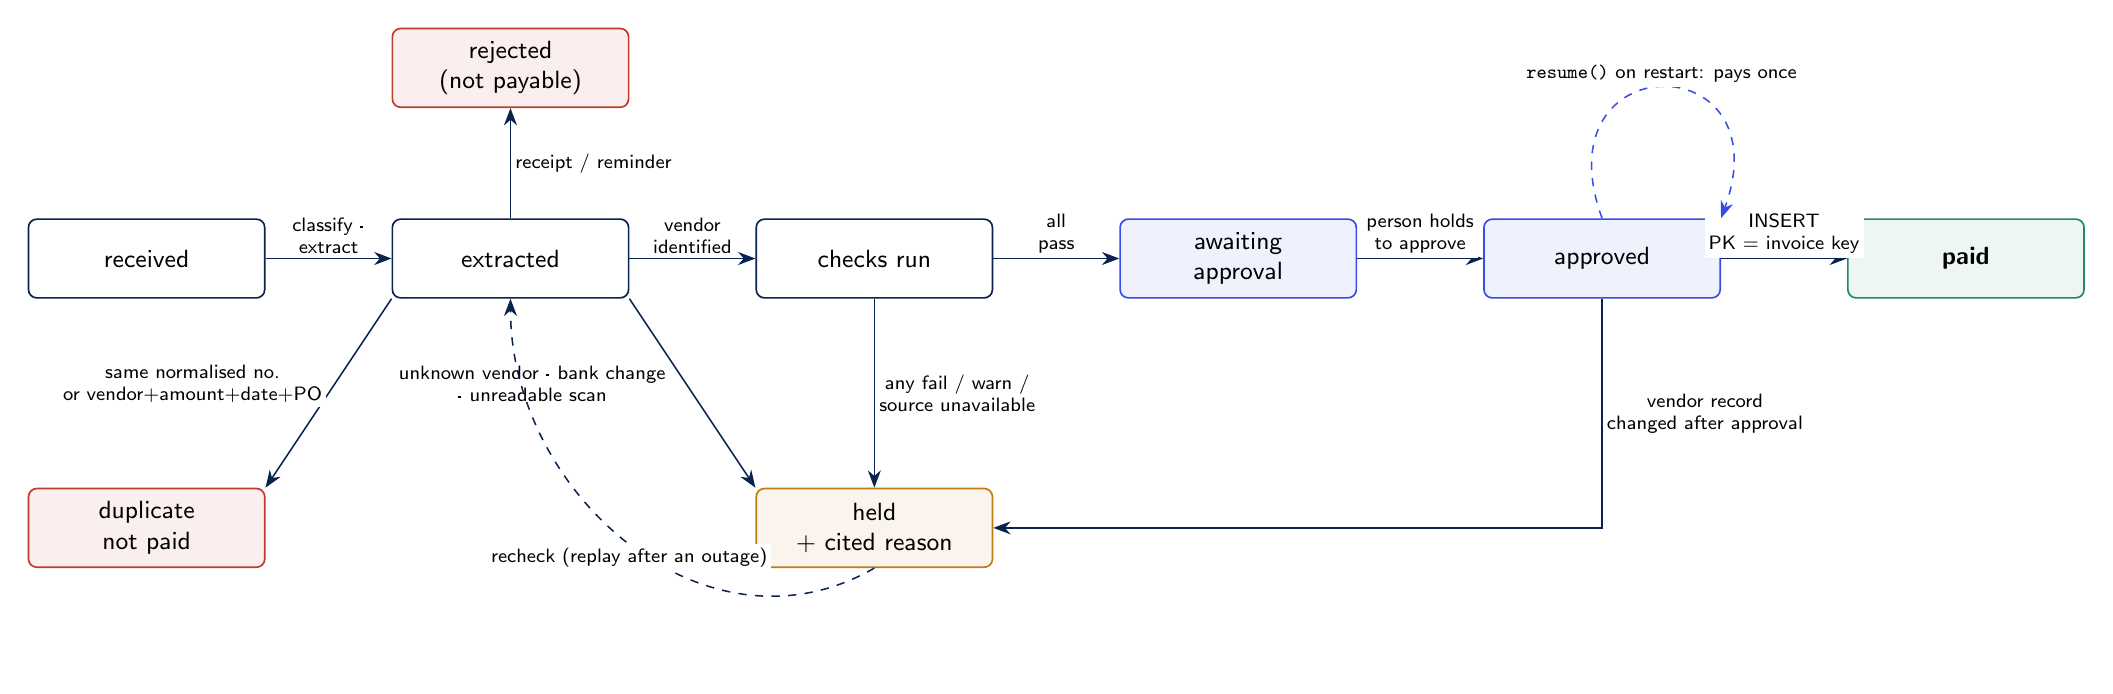
\begin{tikzpicture}[node distance=10mm and 16mm]
\node[s] (rec) {received};
\node[s,right=of rec] (ext) {extracted};
\node[s,right=of ext] (ver) {checks run};
\node[wait,right=of ver] (aw) {awaiting\\approval};
\node[wait,right=of aw] (ap) {approved};
\node[ok,right=of ap] (paid) {\textbf{paid}};
\node[no,below=24mm of rec] (dup) {duplicate\\not paid};
\node[no,above=14mm of ext] (rej) {rejected\\(not payable)};
\node[hold,below=24mm of ver] (held) {held\\+ cited reason};
\draw[arr] (rec) -- node[e,above]{classify \textperiodcentered{}\\extract} (ext);
\draw[arr] (ext) -- node[e,above]{vendor\\identified} (ver);
\draw[arr] (ver) -- node[e,above]{all\\pass} (aw);
\draw[arr] (aw) -- node[e,above]{person holds\\to approve} (ap);
\draw[arr] (ap) -- node[e,above]{INSERT\\PK = invoice key} (paid);
\draw[arr] (ext.south west) -- node[e,pos=.45,left=1mm]{same normalised no.\\or vendor+amount+date+PO} (dup.north east);
\draw[arr] (ext) -- node[e,right]{receipt / reminder} (rej);
\draw[arr] (ver) -- node[e,right]{any fail / warn /\\source unavailable} (held);
\draw[arr] (ext.south east) -- node[e,pos=.45,left=2mm]{unknown vendor \textperiodcentered{} bank change\\\textperiodcentered{} unreadable scan} (held.north west);
\draw[arr] (ap) |- node[e,pos=.25,right]{vendor record\\changed after approval} (held);
\draw[arr,dashed] (held.south) to[out=-150,in=-90,looseness=1.1] node[e,below,pos=.5]{recheck (replay after an outage)} (ext.south);
\draw[arr,dashed,draw=blue] (ap.north) to[out=110,in=70,looseness=4] node[e,above]{\texttt{resume()} on restart: pays once} (ap.north east);
\end{tikzpicture}
\end{document}
